\section{Various Pupil Functions}

The selection of an arbitrary pupil shape and size requires the variation of only the Pupil Function given in Section \ref{sec:FrApprox} Equation \ref{PupilFunction}.  It can be specified discretely, however the discrete sampling should be at least as small as the wavefront sampling.  The result for a square pupil and a round pupil are shown below in Figure \ref{fig:Pupils}.

\begin{figure}[H]
    \subfloat[Circular pupil function of diameter D: $D = 300 \mu m$, $f = 18 mm$, $\lambda = 630 nm$]{%
    	\includegraphics[width=.48\linewidth]{figures/CircularAperture.pdf}
   	}
    \hfill
	\subfloat[Square pupil function of width D: $D = 300 \mu m$, $f = 18 mm$, $\lambda = 630 nm$]{%
    	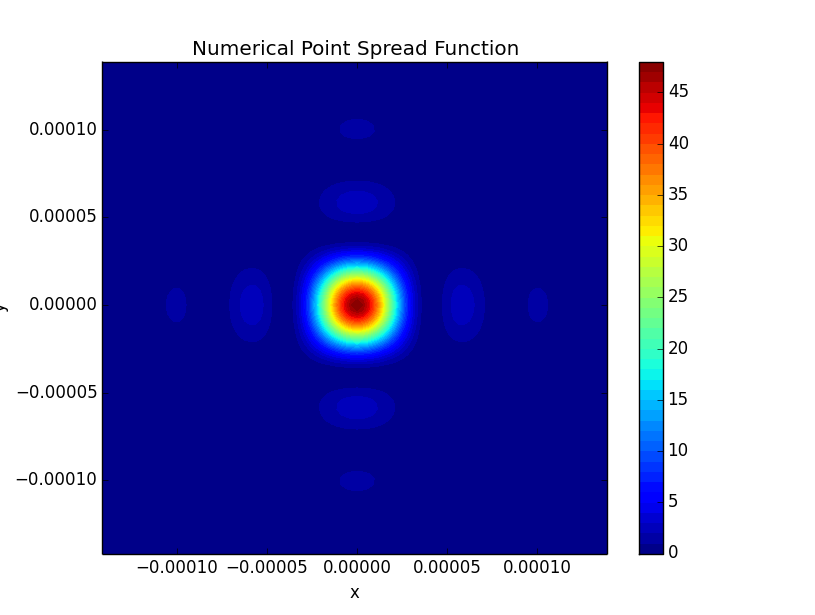
\includegraphics[width=.48\linewidth]{figures/SquareAperture.pdf}
   	} 
	\caption{Intensity Distribution for different pupil shapes.}
	\label{fig:Pupils}
\end{figure}

The intensity distribution for the square pupil shows a similarity to the diffraction pattern for a slit along the x and y axes.  The central peak is a rounded-square with fringes out along the x, y axes and in the diagonals.  